\documentclass[12pt]{article}

\usepackage{geometry,calc}
\usepackage{amsmath,amssymb,hyperref}

\def\quiztitle{Graded Problem 1\color{red} KEY}
\def\quizsubtitle{Math 4B,\qquad Spring 2017,\qquad Dr. Paul}
\pagestyle{empty}

\geometry{body={6.5in, 9in}, left=1in, top=1in}
\input{../../AxesFunction.tex}

\everymath{\displaystyle}

\begin{document}

%\hfill Student Name: \rule{2in}{.1pt}\\

%\hfill Section Time (e.g. 8am): \rule{2in}{.1pt}\\

\begin{center}
{\Huge \quiztitle}
\vskip.1in
{\large \quizsubtitle}
\end{center}
{\color{red} Grade out of 5 point (one bonus point possible). DO NOT DISTRIBUTE}
\begin{enumerate}



 \item Recall our model for disease spread from class:
 $$\begin{array}{rcl}
 S'&=&-10^{-5} S I\\
 I'&=&10^{-5}SI -\frac{1}{14}I\\
 R'&=&\frac{1}{14}I
 \end{array}$$
 \begin{enumerate}
  \item {\color{red} (1 point)} With the initial data $S(0)=45400$, $I(0)=2100$, $R(0)=2500$, use a computer program like Excel, Google Sheets, or Python to implement Euler's method and predict how many people are susceptible, infected, and resistant after 30 days. Create a graphic showing what happens over the course of these 50 days. 
  
  {\color{red} You don't need to check this carefully. Below are the sample graphs I showed them. If they obviously just used screenshot of one of these, they shouldn't get credit.}
  
  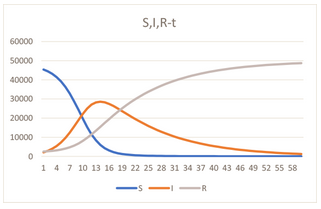
\includegraphics[width=.3\textwidth]{SIRGraphs} 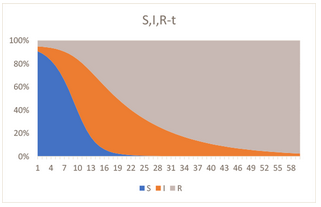
\includegraphics[width=.3\textwidth]{SIRPercents} 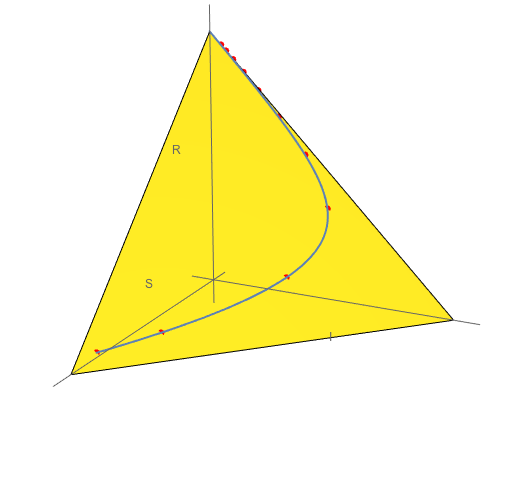
\includegraphics[width=.3\textwidth]{SIRPhase}
  
  \item {\color{red} (1 point)} Even though $S$ and $R$ are functions of time, is still makes sense to think about how these two quanities relate to one another. Using chain rule from Calc 1, we know $\frac{dS}{dR}\frac{dR}{dt}=\frac{dS}{dt}$. Assuming $I\neq0$, solve for $\frac{dS}{dR}$ and then find $S$ as a function of $R$.
  
  {\color{red} $$\frac{dS}{dR}=-\frac{10^{-5}SI}{I/14}=-0.00014S$$
  $$S(R)=Ce^{-0.00014R},\quad S(2500)=45400$$
  $$S(R)\approx 64426e^{-0.00014R}$$}
  
  \item (Bonus{\color{red} (1 point)}) Does everyone on the island eventually get sick? Or do some susceptible people remain? Explain your answer both numerically (using the data from part a) and analytically (using your equation from part b).
  
  {\color{red} For half a point, they can explain numerically, and note that $S$ seems to stabilize at 29 or 30. For the other half point, they can realize that if $S(R)\approx 64426e^{-0.00014R}$ and $S+R<50000$, then $S>29$.}
 \end{enumerate}
 

 \item We now consider a NEW model for disease spread with \emph{immunity loss}. We use the same model as before, with transmission coefficient $4\times 10^{-5}$ and recovery coefficient $0.2$, but with additional provision that on any particular day, a Resistant person has a $3\%$ chance of becoming Susceptible.
 
 \begin{enumerate}
  \item {\color{red} (1 point)} Adapt the model discussed in class to include the effect of the immunity loss. 
  
  {\color{red} $$S'=-4\times 10^{-5}SI+0.03R,\quad I'=4\times 10^{-5}SI-0.2I,\quad R=0.2I-0.03R$$}
  \item {\color{red} (Do not grade.)} Under what circumstances will the number of recovered individuals decrease?
  \item {\color{red} (1 point)} Is there a set of initial data (with 50,000 people total) for which the numbers of Susceptible, Infected, and Resistant people stay constant (i.e. an \emph{equilibrium} or \emph{steady state})?
  {\color{red} $$S=5000, I\approx5870, R\approx39130$$}
 \end{enumerate}

 
 \item {\color{red} (1 point)} Create a system of differential equations that would model a zombie outbreak. You can use the S-I-R model as a starting point, but the rules will probably be different (e.g. there may be an ``undead'' category). Write a few sentences explaining your model. Which rates of change are affected by which variables? What is the long-term behavior of your system?
 
 {\color{red} Anything that isn't utter nonsense gets credit here.}

\end{enumerate}



\end{document}